\subsection{Testauswertung}
In diesem Unterkapitel erkläre ich die Implementierung der Input Control und auf welche Art und Weise sie auf Benutzereingaben reagiert. Danach zeige ich auf, was mir bei den Performance Tests aufgefallen ist und hebe bestimmte Testergebnisse hervor.

\subsubsection{Verhalten der Input Control}
Während der Input Control-Tests habe ich absichtlich einige Leerzeichen in die Eingaben eingefügt, um in der Output-Korrektur zu zeigen, dass der white space entfernt wird. Invalid input entsteht, wenn keine Zahlenwerte in input fields eingegeben wurden, die eine Zahl erwarten. In dem Fall bleibt die Eingabe stehen bis sie verändert wird. Solange invalid input im input field vorhanden ist, ist die zugehörige Operation blockiert. Floats mit Kommas zählen ebenfalls zu invalid input. Stattdessen muss die englische Schreibweise mit Punkt eingetippt werden. Eine Ausnahme von blockierten Operationen stellt der pageCounter dar. In diesem input field wird beim Scrollen das invalid input automatisch entfernt und mit der aktuellen Seitenzahl der im Viewport dargestellten Seite aktualisiert. Die textarea für den benutzerdefinierten Text akzeptiert alle Unicode-Zeichen, falls die Schriftart Unicode darstellen kann. Die 14 Standard-Fonts Times Roman (normal, bold, italic), Helvetica (normal, bold, italic), Courier (normal, bold, italic), ZapfDingbats (normal) und Symbol (normal) unterstützen kein Unicode, was ein Resultat der langen Tradition der PDF-Spezifikation ist. Ich habe lediglich alle Times Roman-, Helvetica- und Courier-Schriftschnitte zur Verwendung freigegeben. Times Roman, Helvetica und Courier implementieren die WinAnsi-Encodierung und ZapfDingbats und Symbol verwenden ihre eigenen spezialisierten Encodings mit 203 und 194 Zeichen \cite{pdf-lib}. Daher sollte zur Sicherheit immer ein benutzerdefinierter Font verwendet werden. Ansonsten wird ein Fehler geworfen, der in Screenshot \ref{fig:font-error} gezeigt ist.

\begin{figure}[!htbp]
	\centering
	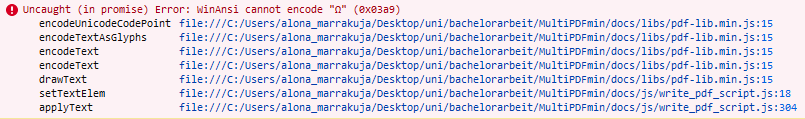
\includegraphics[width=1\textwidth]{"images/font-error.png"}
	\caption{Auftretende Fehlermeldung, wenn der User bei Verwendung eines PDF-Standard-Fonts versucht in die textarea ein Omega-Zeichen einzufügen}
	\label{fig:font-error}
\end{figure}

Das input field Zoom akzeptiert einen Integer mit oder ohne Prozentzeichen. Falls kein Prozentzeichen eingetippt wurde, wird es automatisch hinzugefügt. Das Prozentzeichen soll die Zoomfunktionalität im GUI-Layout verdeutlichen. Liegt eine Zahl unter dem minimalen Wertebereich, so wird die Eingabe auf die unterste Schwelle korrigiert. Falls die Zahl über dem maximalen Wertebereich liegt, wird sie auf die oberste Schwelle substituiert. Sowohl bei Integer als auch bei Float input fields können bei Werten zwischen –1 und 1 die Null vor dem Dezimalpunkt weggelassen oder auch mehrere Nullen geschrieben werden. Im Falle eines Integers wird die Eingabe intern als 0 interpretiert. Hingegen wird bei einem Float die 0 ergänzt bzw. zu einer 0 zusammengefasst. Wird ein Float in einem Integer input field eingegeben, so wird immer abgerundet, d.h. die Zahlen hinter dem Dezimalpunkt werden entfernt. Die Seitenlisten im Splitter und in den Selection Filter im Editor löschen den Inhalt des input fields bei invalid input. Die letzte Seite eines PDFs im Splitter gilt ebenfalls als invalid input. Außerdem werden Duplikate entfernt und die Seitenzahlen in aufsteigender Reihenfolge sortiert. Die korrigierte Eingabe substituiert die Benutzereingabe, falls die Eingabe valide war. 

\subsubsection{Performance-Test-Beobachtungen}
Wird eine PDF-Datei in einem beliebigen Modul geöffnet und gleichzeitig die geöffnete Datei auf der Festplatte gelöscht, so ergibt sich keine Fehlermeldung in der Anwendung. Darüber hinaus stürzt die Anwendung nicht ab oder friert ein. Ursache dessen ist, dass die Darstellung des PDF-Dokuments in der Anwendung unabhängig von der Datei auf der Festplatte ist. Die Testergebnisse der Performance Tests zeigen, dass die Renderdauer maßgeblich von der Dateigröße abhängt. Das größte PDF mit 167,05 MB hat nur 50 Seiten, jedoch gehört es zu den PDFs, die für das Rendern im Reader den größten Zeitraum benötigte. Die maximale Renderdauer von 1,67 Minuten habe ich im PDF mit 850 Seiten vorgefunden. Es forderte sogar ungefähr 1 Minute mehr Zeit als das leere PDF mit 5000 Seiten, welches ich im Creator erstellt hatte. PDFs mit mehr als 1000 Seiten gehen in den Sekundenbereich.
\par 
Bei den Creator Testfällen fällt auf, dass das PDF-Format sich kaum auf die Ausführungszeit auswirkt. Eine Seite mit dem maximal unterstützten Format liegt im Bezug auf die Speichergröße im Bytebereich. Es wird deutlich, dass die PDF-LIB den Speicherplatzbedarf für leere PDFs optimiert hat. Ebenfalls dauert die Ausführung der Downloadfunktion für die maximale Anzahl an Seiten nur wenige Sekunden. 
\par
In den Testresultaten des Editors fällt auf, dass die Einbettung von 20 Texts oder Drawings ungefähr gleich viel Speicherplatz belegen. Bei Verwendung von 20 Images steigt die Outputdatei auf über 10 MB an. Hingegen erzeugen Text, Drawings oder Shapes über 8,6 MB. Sogar die Einbettung von Text und Shapes ist weniger speicherintensiv als die Einbettung von Images. Die Ausführungszeit steigt mit Anzahl der eingebetteten Elementen quasi proportional. Alle 4 Elementtypen benötigen über 1 Sekunde, um heruntergeladen zu werden. Zeitlich gesehen ist die Einbettung der einzelnen Elemente im Bezug auf ihre Elementart sehr ähnlich. Bei einer gedrehten Seite ist der Speicherplatzunterschied zum source PDF im vernachlässigbaren einzelnen Bytebereich. Im nächsten Kapitel diskutiere ich, welche Funktionen in der PDF Web App ausbaufähig sind und welche Features zukünftig geplant sind.